\chapter{Background}
\section{Background Research}
\subsection{Federated Learning}
% Introduce federated learning
Many modern machine learning algorithms require large volumes of diverse data to achieve optimal performance. Real-world data is often distributed among multiple organizations that are unable to share it with each other due to privacy regulations such as GDPR \cite{gdpr}, reducing the amount of data available to train models on and negatively impacting trained performance \cite{data_volume}. Federated Learning (FL) \cite{survey_on_fed_learning} is a technique in machine learning that aims to train a single model using all available data across organizations without requiring any data to be shared among them. \\

% Intro on how fed learning works and different types
There are a multitude of published FL frameworks \cite{fed_table_survey}, each with different merits and drawbacks for certain use cases. Federated Averaging (FedAvg) \cite{fed_learning} is a commonly used yet simple framework, which splits training into iterations where three steps take place:
\begin{enumerate}
	\item A copy of the current model is sent to each agent
	\item Each agent performs some training with their copy of the model and their own private data
	\item The trained models from each agent are sent back to the server to aggregate into a global model
\end{enumerate}
The global model improves over time, and after a certain number of steps, the training is complete and the global model is the final output. \\

% Specify why federated learning is better than conventional learning
As it does not require data to be shared between agents, FL is naturally beneficial for privacy sensitive tasks compared to conventional machine learning where the data is aggregated in a central location \citeme. Additionally, as FL performs training on multiple agents in parallel, it can make better use of available training resources in situations where processing power is distributed among multiple nodes \citeme.

% federate distributed
One branch of FL is distributed federated learning (DFL). This algorithm works in a very similar way to FL, but replaces the central server with an elected leader in a network of agents \cite{leaderelec_car}. DFL has been shown to increase fault tolerance and security over FL.


\subsection{Swarm Learning}
% Introduce swarm learning
Swarm learning (SL) \cite{swarm_learning} is a subcategory of FL which operates in a completely distributed and decentralised manner. SL still allows a network of agents to collaborate to learn a shared model, but at no point is a central server used or a leader chosen. In contrast to FL, SL methods usually use a blockchain based system to coordinate a global model.

\begin{figure}[h]
	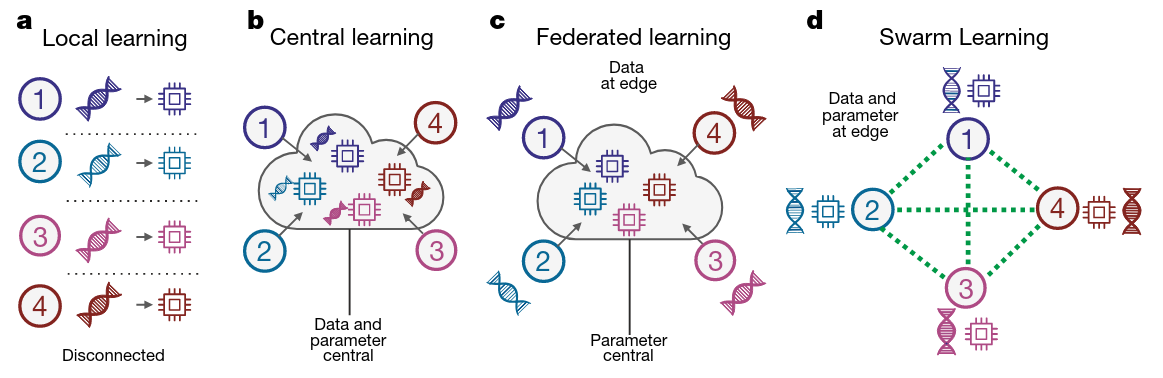
\includegraphics[width=\linewidth]{sl}
	\caption{Diagram of swarm learning compared to other type of learning taken from \cite{swarm_learning}}
	\label{fig_learning}
\end{figure}


In SL, agents learn in a similar fashion to FL in training steps. However, the agents do not need to have their training steps synchronised. Following are the typical training steps of a swarm learning agent:
\begin{enumerate}
	\item An agent obtains a copy of the current model from the blockchain
	\item The agent performs some training with their copy of the model and their own private data
	\item The updated model is merged with the current model on the blockchain and sent back to the blockchain for other agents to use
\end{enumerate}
The model on the blockchain will improve over time, and after a certain number of steps the blockchain model is the final output. \\

% Specify why swarm learning is better than conventional learning or federated learning
SL exhibits many of the same benefits of FL over conventional learning, but it also improves upon FL in some aspects. As is often the case when comparing decentralised algorithms to their centralised counterparts \cite{swarm_resil}, the absence of a central server makes SL more resilient to failures than centralized FL approaches such as FedAvg. The lack of a leader election protocol also means that SL may be better suited to tasks where networks of agents are sparsely connected, as leader election in dynamic networks is a complex problem and can add large amounts of overhead \cite{leaderelection}. Additionally, the removal of the need for a server in SL reduces the likelihood of performance bottlenecks for very large swarms.

\subsection{Challenges for Federated and Swarm Learning}
There are numerous challenges associated with implementing FL or SL compared to conventional learning systems. Some of the common challenges are described below:

\subsubsection{Training Overhead}
Since FL and SL require communication between multiple agents, there is an inherent overhead cost associated with data transfer time and synchronization of agents. Additionally, the centralization of FL can result in server bottlenecking. This is an area where SL offers an improvement over conventional FL. One potential solution to reduce bottlenecks is to divide the agents into groups, each with its own central server, and enable those servers to communicate with a core server \cite{multi_center_fed_learning}. This has the potential to reduce the burden on the central server and improve overall performance.

\subsubsection{Unevenly Distributed Labels and Features - Non-IID Data}
When a dataset is collected from various sources and locations, it will have a specific distribution of features and labels. However, the distribution of these features and labels may differ among the different sources from which it was collected, meaning the data is referred to as non-iid. For example, a dataset containing security camera footage of car and bus accidents may have more of one type of accident at some locations than others (labels). The cameras at different locations may also have varying brightness or contrast settings (features). This can negatively impact the training of SL and FL algorithms \cite{noniid_bad} because each agent is effectively proposing a solution to a different problem than the rest. There is a significant amount of research being conducted on this topic, with various approaches being proposed \cite{survey_noniid}.

One approach is to partition agents into different clusters, where each member of a cluster communicates with the same server. The servers at the centre of each cluster will perform FL with their respective agent, but still synchronise the cluster model to all other cluster servers \cite{multi_center_fed_learning}. This allows each sub-cluster to develop its own modified version of the global model to suit its needs.

A different approach is to use batch normalisation layers on each agent \cite{fedbn}, which adds a degree of standardisation to activations in the network. This method is focussed on non-iid features as opposed to non-iid labels, and has shown to have excellent results as opposed to a multitude of other FL techniques.

\subsubsection{Sparsely Connected Networks}
For FL, ideally every agent would be able to have direct communication with the central server. Similarly for SL in the best case, every agent would have direct communication with every other agent. However, these cases are rarely ever realised. The effect of having a sparsely connected network is more detrimental to FL than SL mainly because FL needs server communication, but SL and blockchain have been proven to work in sparse settings. This can however still slow the training of SL.

\subsubsection{Data Transfer Limits}
In the real world, it is sometimes not possible to transfer entire models between agents on a regular basis, due to data transfer limits. It has been proposed that a possible solution could be to use FedAvg, but only transfer segments of the network at each training step \cite{gossip_learning}. This approach outperformed FedAvg by a factor of between 2.25 and 3.01 with respect to training speed, due to the removal of the central server bottleneck and reduced data transferred \cite{gossip_learning}[section.~5.2].

\subsubsection{Low Processing Power Agents}
FL and SL are promising techniques for robotic systems \cite{fed_in_robotics} and Internet-of-Things (IoT) devices \cite{fed_iot}. However, these systems often do not have the same high level of processing power as a central machine learning server. For this reason, it is imperative that FL and SL systems are as efficient as possible with the results of their training as to minimise the loss caused by reduction in processing power.

